\documentclass[compress, containsverbatim,mathserif, xcolor=dvipsnames, unicode]{beamer}


%tema
\usetheme{Antibes}
\usecolortheme[named=Maroon]{structure}
\usecolortheme{beaver}
\setbeamercolor{titlelike}{fg=black, bg=purple}
\setbeamercolor{palette primary}{fg=pink, bg=purple}
\setbeamercolor{palette secondary}{fg=purple, bg=pink}
\setbeamercolor{palette tertiary}{bg=purple, fg=black}
\setbeamercolor{palette quaternary}{bg=purple, fg=black}
\setbeamercolor{frametitle}{bg=purple}
\setbeamercolor{block body}{bg=pink, fg=black}
\setbeamercolor{block title}{bg=purple, fg=white}
\setbeamertemplate{itemize item}{\color{purple}$\blacksquare$}
\setbeamertemplate{itemize subitem}{\color{purple}$\blacksquare$}
\setbeamercolor{item projected}{bg=purple,fg=white}
\setbeamercolor{section in toc}{fg=purple,bg=white}





% zbog srpskog
\usepackage[serbian]{babel}
\usepackage[utf8]{inputenc}
\usepackage[T2A]{fontenc}

% za matematiku
\usepackage{amsmath}
\usepackage{amssymb}
\usepackage{fontawesome5}

\usepackage{xcolor}

\newtheorem{primer}{Primer}[section]

\title{Optimizacije kroz GCC, LLVM i Native Image}
\author{Tamara Stojković, Emilija Stošić, Teodora Isailović}
\institute{Metodologija stručnog i naučnog rada \\ Matematički fakultet \\ Univerzitet u Beogradu}
\date{
	\footnotesize{Beograd, decembar 2022.}	
}

\begin{document}

\begin{frame}
\titlepage

\begin{figure}[h!]
    \centering
    \begin{flushleft}
    
\includegraphics[width=15mm]{logo.png}
    \end{flushleft}
\end{figure}
\end{frame}

\begin{frame}{Sadržaj}
\tableofcontents
\end{frame}

\section{Uvod}
\begin{frame}{Uvod}
\vspace{\baselineskip}
\begin{itemize}
	\item Optimizacija - tehnika transformacije dela programa, sa ciljem poboljšanja performansi koda
    \item Oblast u kojoj se danas vrši većina istraživanja kompajlera
    \item Kompajleri - različiti nivoi optimizacije
	\item Na nivoima kompromisi između mera - kvalitet koda, veličina koda, vreme kompilacije
    \item Izbor kompajlera i nivoa optimizacije zavise od konkretnog programa
\end{itemize}
\end{frame}



\section{Osnovna podela optimizacija}
\subsection{Optimizacije međukoda}
\begin{frame}{Lokalne optimizacije}
    
    \begin{itemize}
        \item Razlikujemo: lokalne, globalne i međuproceduralne
        \item  \textcolor{purple}{Lokalne optimizacije} služe za ubrzavanje malih delova neke funkcije, najlakše za izvođenje
        \item Tehnike lokalne optimizacije koje razlikujemo: 
                \begin{itemize}
                    \item Eliminacija čestih podizraza
                    \item Slaganje konstanti
                    \item Propagacija kopija
                    \item Smanjenje snage operatora
                    \item Eliminacija mrtvog koda
                    \item Algebarsko pojednostavljenje i reasocijacija
                    \item Kompozicija lokalnih transformacija
                \end{itemize}
        \end{itemize}
\end{frame}


\begin{frame}{Globalne i međuproceduralne optimizacije}
    \begin{itemize}
        \item \textcolor{purple}{Globalne optimizacije} primenjuju se na jednu po jednu funkciju, slične lokalnim
        \item Globalne optimizacije koje razlikujemo: 
                \begin{itemize}
                    \item Globalna eliminacija mrtvog koda
                    \item Globalno propagiranje konstanti
                    \item Globalna eliminacija čestih podizraza
                    \item Optimizacija kretanje koda
                    \item Pomeranje invarijantog koda
                    \item Parcijalna eliminacija suvišnosti
                \end{itemize}
        \item \textcolor{purple}{Međuproceduralna optimizacija } - radi na celokupnom grafu kontrole toka
        \item Vrši se na nivou celog programa tj. više funkcija 
        \item Najpoznatija tehnika je uvlačenje definicija funkcija 
        \end{itemize}
\end{frame}


\subsection{Optimizacije koda}
\begin{frame}{Optimizacije koda}
    
    \begin{itemize}
        \item Optimizovani međukod se prevodi u asemblerski tj. mašinski kod - faza generisanja
        \item  Bitne su specifične karakteristike mašine
        \item Razlikujemo  sledeće tehnike: 
                \begin{itemize}
                    \item Optimizacija redosleda instrukcija - obuhvata fazu odabira instrukcija, alokacije registara i raspoređivanja instrukcija
                    \item Optimizacija upotrebom keša - zasniva se na prostornoj i vremenskoj lokalnosti, cilj da bude što bolja
                \end{itemize}
        \end{itemize}
\end{frame}







%samo je testirano dodavanje slika -ubacite koju hocete i kako hocete i koliko po slajdu
%\section{dodati naziv}
\begin{frame}{GCC optimizacija} %promeniti sve
    \begin{figure}[h!]
        \begin{center}
       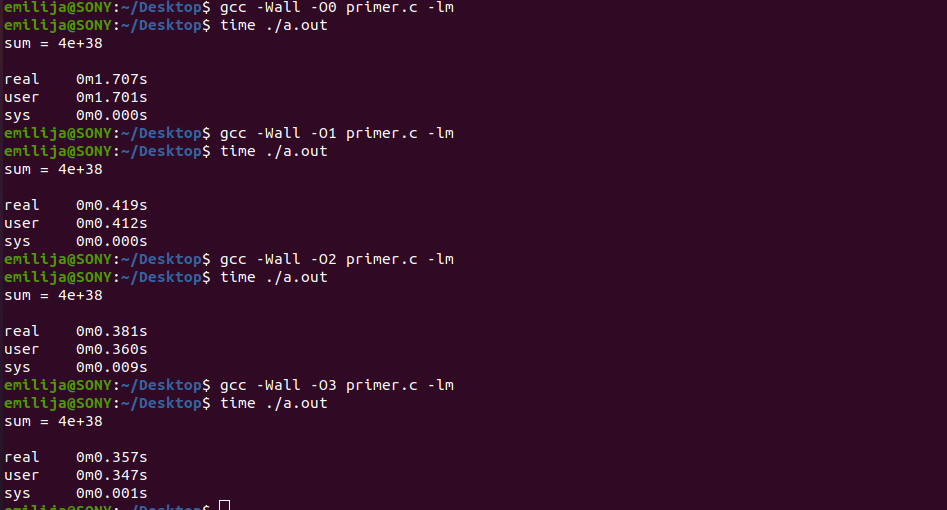
\includegraphics[scale = 0.2]{../pics/test.png}
       \end{center}
       \caption{Rezultati optimizacije kod GCC kompajlera}
    \end{figure} 
\end{frame}


\end{document}

    
